%#################################################################
\chapter{Metodologia da Pesquisa}\label{metodologiaPesquisa}
%#################################################################

Este capítulo aborda a metodologia de pesquisa adotada para a execução deste estudo. 
Na Seção \ref{sec:TiposPesquisa} são elencadas as classificações dos tipos de pesquisa. 
Os desenhos de pesquisa do \ac{TCC} I e II utilizados para a execução da pesquisa são apresentados na Seção \ref{sec:DesenhoPesquisa} e, em seguida, na Seção \ref{sec:licMetodo} as lições do capítulo são pontuadas.

%#################################################################
\section{Classificação de Pesquisa} \label{sec:TiposPesquisa}
%#################################################################

Segundo \citeonline{Wazlawick:2017}, as monografias geralmente possuem um capítulo para a elucidação da metodologia. 
Contudo, analisando-se semanticamente o termo, a metodologia seria o estudo dos métodos. 
Apesar do uso corrente, linguisticamente seria mais correto afirmar que um trabalho científico individualmente tem um método de pesquisa, ou desenho de pesquisa, utilizando abordagens, técnicas e procedimentos diversos combinados.

Em geral, para que um estudo possa ter maior confiança no que diz respeito ao rigor científico, é imprescindível que sejam identificadas as atividades e técnicas necessárias que possibilitem a se chegar no objetivo proposto \cite{Peffers:2007}. A \autoref{fig:ClassificacaoPesquisa} mostra a classificação desse estudo mediante sua natureza, abordagem, objetivos e procedimentos. 

%\begin{figure}[!htb]
%	\centering
%	\caption{Classificação da Pesquisa}
		%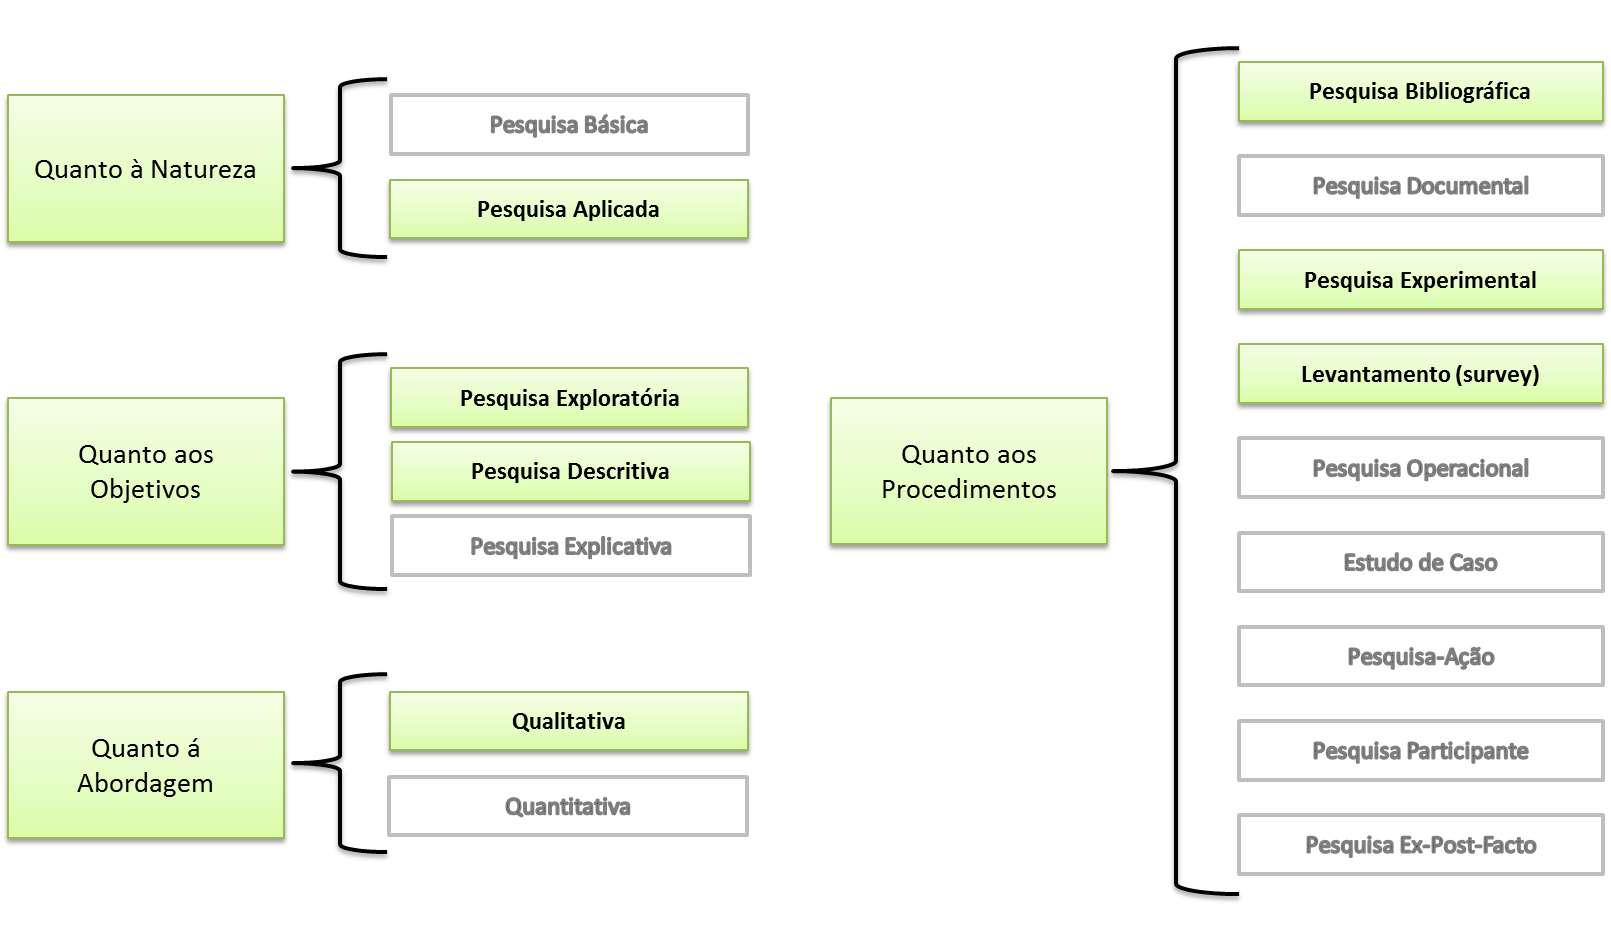
\includegraphics[width=\textwidth]{img/ClassificacaoPesquisa.png}
%	\fonte{Adaptado de \citeonline{Prodanov:2013}.}
%	\label{fig:ClassificacaoPesquisa}
%\end{figure}


\begin{figure}[!htb]
\centering
\caption{Classificação da Pesquisa.}


\tikzset{every picture/.style={line width=0.75pt}} %set default line width to 0.75pt        

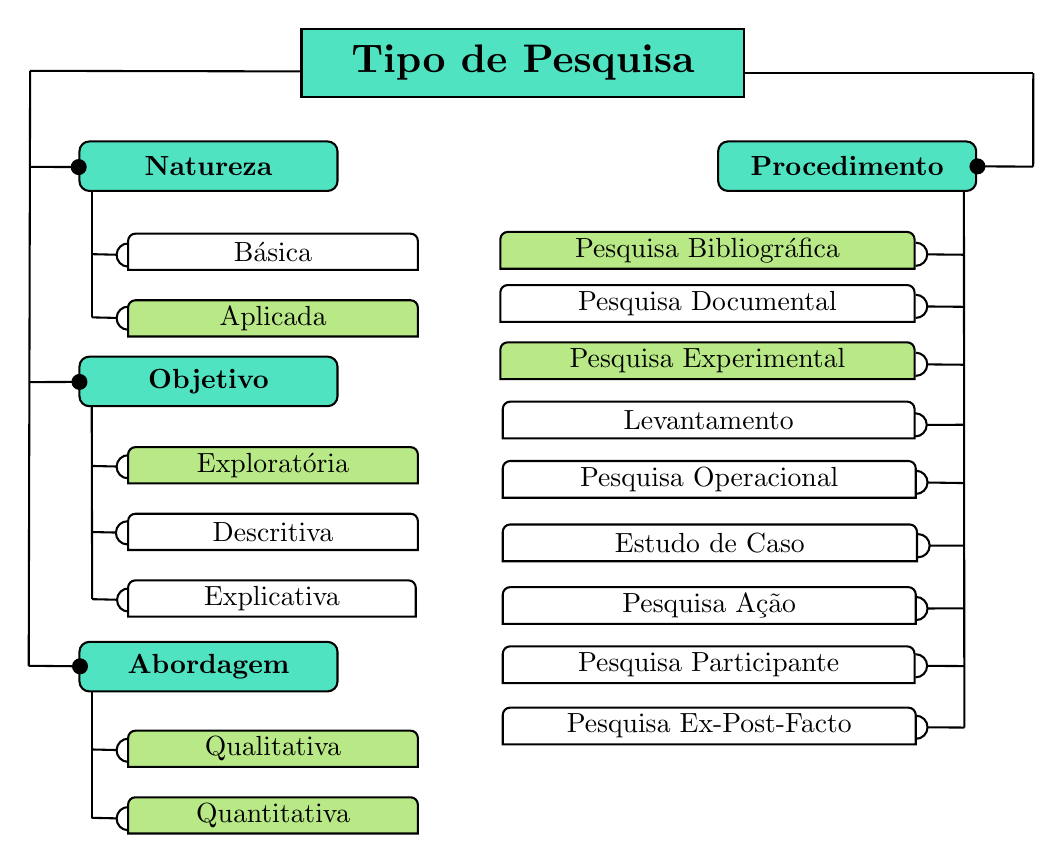
\begin{tikzpicture}[x=0.75pt,y=0.75pt,yscale=-1,xscale=1]
%uncomment if require: \path (0,575); %set diagram left start at 0, and has height of 575

%Shape: Rectangle [id:dp4577118281096286] 
\draw  [fill={rgb, 255:red, 80; green, 227; blue, 194 }  ,fill opacity=1 ] (224.94,20) -- (438.21,20) -- (438.21,52.92) -- (224.94,52.92) -- cycle ;
%Rounded Rect [id:dp34276139041627407] 
\draw  [fill={rgb, 255:red, 80; green, 227; blue, 194 }  ,fill opacity=1 ] (117.95,320.19) .. controls (117.95,317.55) and (120.09,315.42) .. (122.73,315.42) -- (237.49,315.42) .. controls (240.13,315.42) and (242.27,317.55) .. (242.27,320.19) -- (242.27,334.51) .. controls (242.27,337.14) and (240.13,339.28) .. (237.49,339.28) -- (122.73,339.28) .. controls (120.09,339.28) and (117.95,337.14) .. (117.95,334.51) -- cycle ;
%Rounded Rect [id:dp8849258160693669] 
\draw  [fill={rgb, 255:red, 80; green, 227; blue, 194 }  ,fill opacity=1 ] (117.95,79.08) .. controls (117.95,76.45) and (120.09,74.31) .. (122.73,74.31) -- (237.49,74.31) .. controls (240.13,74.31) and (242.27,76.45) .. (242.27,79.08) -- (242.27,93.4) .. controls (242.27,96.04) and (240.13,98.17) .. (237.49,98.17) -- (122.73,98.17) .. controls (120.09,98.17) and (117.95,96.04) .. (117.95,93.4) -- cycle ;
%Rounded Rect [id:dp6071364324721369] 
\draw  [fill={rgb, 255:red, 80; green, 227; blue, 194 }  ,fill opacity=1 ] (117.95,182.77) .. controls (117.95,180.13) and (120.09,178) .. (122.73,178) -- (237.49,178) .. controls (240.13,178) and (242.27,180.13) .. (242.27,182.77) -- (242.27,197.09) .. controls (242.27,199.72) and (240.13,201.86) .. (237.49,201.86) -- (122.73,201.86) .. controls (120.09,201.86) and (117.95,199.72) .. (117.95,197.09) -- cycle ;
%Rounded Rect [id:dp4106241999835438] 
\draw  [fill={rgb, 255:red, 80; green, 227; blue, 194 }  ,fill opacity=1 ] (425.68,79.08) .. controls (425.68,76.45) and (427.81,74.31) .. (430.45,74.31) -- (545.22,74.31) .. controls (547.85,74.31) and (549.99,76.45) .. (549.99,79.08) -- (549.99,93.4) .. controls (549.99,96.04) and (547.85,98.17) .. (545.22,98.17) -- (430.45,98.17) .. controls (427.81,98.17) and (425.68,96.04) .. (425.68,93.4) -- cycle ;
%Rounded Same Side Corner Rect [id:dp2840400712193636] 
\draw  [fill={rgb, 255:red, 255; green, 255; blue, 255 }  ,fill opacity=1 ] (141.39,122.24) .. controls (141.39,120.31) and (142.95,118.75) .. (144.88,118.75) -- (277.5,118.75) .. controls (279.42,118.75) and (280.99,120.31) .. (280.99,122.24) -- (280.99,136.19) .. controls (280.99,136.19) and (280.99,136.19) .. (280.99,136.19) -- (141.39,136.19) .. controls (141.39,136.19) and (141.39,136.19) .. (141.39,136.19) -- cycle ;
%Rounded Same Side Corner Rect [id:dp5724415497830746] 
\draw  [fill={rgb, 255:red, 184; green, 233; blue, 134 }  ,fill opacity=1 ] (141.39,154.33) .. controls (141.39,152.4) and (142.95,150.84) .. (144.88,150.84) -- (277.5,150.84) .. controls (279.42,150.84) and (280.99,152.4) .. (280.99,154.33) -- (280.99,168.28) .. controls (280.99,168.28) and (280.99,168.28) .. (280.99,168.28) -- (141.39,168.28) .. controls (141.39,168.28) and (141.39,168.28) .. (141.39,168.28) -- cycle ;
%Rounded Same Side Corner Rect [id:dp14985801223973771] 
\draw  [fill={rgb, 255:red, 184; green, 233; blue, 134 }  ,fill opacity=1 ] (141.39,225.1) .. controls (141.39,223.17) and (142.95,221.61) .. (144.88,221.61) -- (277.5,221.61) .. controls (279.42,221.61) and (280.99,223.17) .. (280.99,225.1) -- (280.99,239.05) .. controls (280.99,239.05) and (280.99,239.05) .. (280.99,239.05) -- (141.39,239.05) .. controls (141.39,239.05) and (141.39,239.05) .. (141.39,239.05) -- cycle ;
%Rounded Same Side Corner Rect [id:dp37387501315114524] 
\draw  [fill={rgb, 255:red, 255; green, 255; blue, 255 }  ,fill opacity=1 ] (141.39,257.19) .. controls (141.39,255.26) and (142.95,253.7) .. (144.88,253.7) -- (277.5,253.7) .. controls (279.42,253.7) and (280.99,255.26) .. (280.99,257.19) -- (280.99,271.15) .. controls (280.99,271.15) and (280.99,271.15) .. (280.99,271.15) -- (141.39,271.15) .. controls (141.39,271.15) and (141.39,271.15) .. (141.39,271.15) -- cycle ;
%Rounded Same Side Corner Rect [id:dp25377701690503685] 
\draw  [fill={rgb, 255:red, 255; green, 255; blue, 255 }  ,fill opacity=1 ] (141.39,289.28) .. controls (141.39,287.36) and (142.95,285.79) .. (144.88,285.79) -- (276.48,285.79) .. controls (278.41,285.79) and (279.97,287.36) .. (279.97,289.28) -- (279.97,303.24) .. controls (279.97,303.24) and (279.97,303.24) .. (279.97,303.24) -- (141.39,303.24) .. controls (141.39,303.24) and (141.39,303.24) .. (141.39,303.24) -- cycle ;
%Rounded Same Side Corner Rect [id:dp13794965074230814] 
\draw  [fill={rgb, 255:red, 184; green, 233; blue, 134 }  ,fill opacity=1 ] (141.39,361.7) .. controls (141.39,359.77) and (142.95,358.21) .. (144.88,358.21) -- (277.5,358.21) .. controls (279.42,358.21) and (280.99,359.77) .. (280.99,361.7) -- (280.99,375.65) .. controls (280.99,375.65) and (280.99,375.65) .. (280.99,375.65) -- (141.39,375.65) .. controls (141.39,375.65) and (141.39,375.65) .. (141.39,375.65) -- cycle ;
%Rounded Same Side Corner Rect [id:dp46839135503439744] 
\draw  [fill={rgb, 255:red, 184; green, 233; blue, 134 }  ,fill opacity=1 ] (141.39,393.79) .. controls (141.39,391.86) and (142.95,390.3) .. (144.88,390.3) -- (277.5,390.3) .. controls (279.42,390.3) and (280.99,391.86) .. (280.99,393.79) -- (280.99,407.75) .. controls (280.99,407.75) and (280.99,407.75) .. (280.99,407.75) -- (141.39,407.75) .. controls (141.39,407.75) and (141.39,407.75) .. (141.39,407.75) -- cycle ;
%Rounded Same Side Corner Rect [id:dp15982706388592272] 
\draw  [fill={rgb, 255:red, 184; green, 233; blue, 134 }  ,fill opacity=1 ] (320.73,121.47) .. controls (320.73,119.51) and (322.31,117.92) .. (324.27,117.92) -- (516.74,117.92) .. controls (518.7,117.92) and (520.29,119.51) .. (520.29,121.47) -- (520.29,135.64) .. controls (520.29,135.64) and (520.29,135.64) .. (520.29,135.64) -- (320.73,135.64) .. controls (320.73,135.64) and (320.73,135.64) .. (320.73,135.64) -- cycle ;
%Rounded Same Side Corner Rect [id:dp7996243350589711] 
\draw  [fill={rgb, 255:red, 255; green, 255; blue, 255 }  ,fill opacity=1 ] (320.73,147.05) .. controls (320.73,145.1) and (322.31,143.51) .. (324.27,143.51) -- (516.74,143.51) .. controls (518.7,143.51) and (520.29,145.1) .. (520.29,147.05) -- (520.29,161.23) .. controls (520.29,161.23) and (520.29,161.23) .. (520.29,161.23) -- (320.73,161.23) .. controls (320.73,161.23) and (320.73,161.23) .. (320.73,161.23) -- cycle ;
%Rounded Same Side Corner Rect [id:dp30014641980293044] 
\draw  [fill={rgb, 255:red, 184; green, 233; blue, 134 }  ,fill opacity=1 ] (320.73,174.64) .. controls (320.73,172.69) and (322.31,171.1) .. (324.27,171.1) -- (516.74,171.1) .. controls (518.7,171.1) and (520.29,172.69) .. (520.29,174.64) -- (520.29,188.81) .. controls (520.29,188.81) and (520.29,188.81) .. (520.29,188.81) -- (320.73,188.81) .. controls (320.73,188.81) and (320.73,188.81) .. (320.73,188.81) -- cycle ;
%Rounded Same Side Corner Rect [id:dp6116193316770886] 
\draw  [fill={rgb, 255:red, 255; green, 255; blue, 255 }  ,fill opacity=1 ] (321.9,203.23) .. controls (321.9,201.27) and (323.48,199.69) .. (325.44,199.69) -- (516.74,199.69) .. controls (518.7,199.69) and (520.29,201.27) .. (520.29,203.23) -- (520.29,217.4) .. controls (520.29,217.4) and (520.29,217.4) .. (520.29,217.4) -- (321.9,217.4) .. controls (321.9,217.4) and (321.9,217.4) .. (321.9,217.4) -- cycle ;
%Rounded Same Side Corner Rect [id:dp9070606782570514] 
\draw  [fill={rgb, 255:red, 255; green, 255; blue, 255 }  ,fill opacity=1 ] (321.9,231.82) .. controls (321.9,229.86) and (323.48,228.27) .. (325.44,228.27) -- (517.33,228.27) .. controls (519.29,228.27) and (520.87,229.86) .. (520.87,231.82) -- (520.87,245.99) .. controls (520.87,245.99) and (520.87,245.99) .. (520.87,245.99) -- (321.9,245.99) .. controls (321.9,245.99) and (321.9,245.99) .. (321.9,245.99) -- cycle ;
%Rounded Same Side Corner Rect [id:dp026422911508531044] 
\draw  [fill={rgb, 255:red, 255; green, 255; blue, 255 }  ,fill opacity=1 ] (321.9,262.41) .. controls (321.9,260.45) and (323.48,258.86) .. (325.44,258.86) -- (517.92,258.86) .. controls (519.87,258.86) and (521.46,260.45) .. (521.46,262.41) -- (521.46,276.58) .. controls (521.46,276.58) and (521.46,276.58) .. (521.46,276.58) -- (321.9,276.58) .. controls (321.9,276.58) and (321.9,276.58) .. (321.9,276.58) -- cycle ;
%Straight Lines [id:da1670575235577536] 
\draw    (577.5,41.4) -- (577.46,86.44) ;


%Straight Lines [id:da8118950691589346] 
\draw    (123.86,339.28) -- (123.86,400.18) ;


%Straight Lines [id:da17291466732826466] 
\draw    (123.86,201.86) -- (124.07,294.85) ;


%Straight Lines [id:da3815361458832034] 
\draw    (123.86,98.17) -- (123.86,159.07) ;


%Straight Lines [id:da3368611079285959] 
\draw    (123.86,128.62) -- (135.85,128.9) ;
\draw [shift={(135.85,128.9)}, rotate = 1.31] [color={rgb, 255:red, 0; green, 0; blue, 0 }  ][line width=0.75]      (5.59,-5.59) .. controls (2.5,-5.59) and (0,-3.09) .. (0,0) .. controls (0,3.09) and (2.5,5.59) .. (5.59,5.59) ;

%Rounded Same Side Corner Rect [id:dp7931997046212467] 
\draw  [fill={rgb, 255:red, 255; green, 255; blue, 255 }  ,fill opacity=1 ] (321.9,292.6) .. controls (321.9,290.64) and (323.48,289.06) .. (325.44,289.06) -- (517.33,289.06) .. controls (519.29,289.06) and (520.87,290.64) .. (520.87,292.6) -- (520.87,306.77) .. controls (520.87,306.77) and (520.87,306.77) .. (520.87,306.77) -- (321.9,306.77) .. controls (321.9,306.77) and (321.9,306.77) .. (321.9,306.77) -- cycle ;
%Rounded Same Side Corner Rect [id:dp28960792030116966] 
\draw  [fill={rgb, 255:red, 255; green, 255; blue, 255 }  ,fill opacity=1 ] (321.9,321.12) .. controls (321.9,319.17) and (323.48,317.58) .. (325.44,317.58) -- (516.74,317.58) .. controls (518.7,317.58) and (520.29,319.17) .. (520.29,321.12) -- (520.29,335.3) .. controls (520.29,335.3) and (520.29,335.3) .. (520.29,335.3) -- (321.9,335.3) .. controls (321.9,335.3) and (321.9,335.3) .. (321.9,335.3) -- cycle ;
%Rounded Same Side Corner Rect [id:dp49389290024820665] 
\draw  [fill={rgb, 255:red, 255; green, 255; blue, 255 }  ,fill opacity=1 ] (321.9,350.65) .. controls (321.9,348.69) and (323.48,347.11) .. (325.44,347.11) -- (517.33,347.11) .. controls (519.29,347.11) and (520.87,348.69) .. (520.87,350.65) -- (520.87,364.82) .. controls (520.87,364.82) and (520.87,364.82) .. (520.87,364.82) -- (321.9,364.82) .. controls (321.9,364.82) and (321.9,364.82) .. (321.9,364.82) -- cycle ;
%Straight Lines [id:da7075016344613365] 
\draw    (224.94,40.57) -- (94.18,40.3) ;


%Straight Lines [id:da8791469913030159] 
\draw    (94.18,40.3) -- (93.5,326.94) ;


%Straight Lines [id:da6200478575277137] 
\draw    (94.42,86.57) -- (117.59,86.65) ;
\draw [shift={(117.59,86.65)}, rotate = 0.2] [color={rgb, 255:red, 0; green, 0; blue, 0 }  ][fill={rgb, 255:red, 0; green, 0; blue, 0 }  ][line width=0.75]      (0, 0) circle [x radius= 3.35, y radius= 3.35]   ;

%Straight Lines [id:da918961853297364] 
\draw    (94.01,190.26) -- (117.95,190.17) ;
\draw [shift={(117.95,190.17)}, rotate = 359.8] [color={rgb, 255:red, 0; green, 0; blue, 0 }  ][fill={rgb, 255:red, 0; green, 0; blue, 0 }  ][line width=0.75]      (0, 0) circle [x radius= 3.35, y radius= 3.35]   ;

%Straight Lines [id:da08443900683214389] 
\draw    (93.5,326.94) -- (118.21,327.19) ;
\draw [shift={(118.21,327.19)}, rotate = 0.57] [color={rgb, 255:red, 0; green, 0; blue, 0 }  ][fill={rgb, 255:red, 0; green, 0; blue, 0 }  ][line width=0.75]      (0, 0) circle [x radius= 3.35, y radius= 3.35]   ;

%Straight Lines [id:da08124554802054562] 
\draw    (577.5,41.4) -- (438.24,41.4) ;


%Straight Lines [id:da8343656632858758] 
\draw    (577.46,86.44) -- (550.6,86.33) ;
\draw [shift={(550.6,86.33)}, rotate = 180.25] [color={rgb, 255:red, 0; green, 0; blue, 0 }  ][fill={rgb, 255:red, 0; green, 0; blue, 0 }  ][line width=0.75]      (0, 0) circle [x radius= 3.35, y radius= 3.35]   ;

%Straight Lines [id:da5805409911126018] 
\draw    (123.86,159.07) -- (135.85,159.34) ;
\draw [shift={(135.85,159.34)}, rotate = 1.31] [color={rgb, 255:red, 0; green, 0; blue, 0 }  ][line width=0.75]      (5.59,-5.59) .. controls (2.5,-5.59) and (0,-3.09) .. (0,0) .. controls (0,3.09) and (2.5,5.59) .. (5.59,5.59) ;

%Straight Lines [id:da08813150434666617] 
\draw    (123.86,230.66) -- (135.85,230.93) ;
\draw [shift={(135.85,230.93)}, rotate = 1.31] [color={rgb, 255:red, 0; green, 0; blue, 0 }  ][line width=0.75]      (5.59,-5.59) .. controls (2.5,-5.59) and (0,-3.09) .. (0,0) .. controls (0,3.09) and (2.5,5.59) .. (5.59,5.59) ;

%Straight Lines [id:da8789308114642371] 
\draw    (123.52,262.48) -- (135.51,262.75) ;
\draw [shift={(135.51,262.75)}, rotate = 1.31] [color={rgb, 255:red, 0; green, 0; blue, 0 }  ][line width=0.75]      (5.59,-5.59) .. controls (2.5,-5.59) and (0,-3.09) .. (0,0) .. controls (0,3.09) and (2.5,5.59) .. (5.59,5.59) ;

%Straight Lines [id:da3029508317300338] 
\draw    (124.07,294.85) -- (136.06,295.12) ;
\draw [shift={(136.06,295.12)}, rotate = 1.31] [color={rgb, 255:red, 0; green, 0; blue, 0 }  ][line width=0.75]      (5.59,-5.59) .. controls (2.5,-5.59) and (0,-3.09) .. (0,0) .. controls (0,3.09) and (2.5,5.59) .. (5.59,5.59) ;

%Straight Lines [id:da18852599605985843] 
\draw    (123.86,400.18) -- (135.85,400.45) ;
\draw [shift={(135.85,400.45)}, rotate = 1.31] [color={rgb, 255:red, 0; green, 0; blue, 0 }  ][line width=0.75]      (5.59,-5.59) .. controls (2.5,-5.59) and (0,-3.09) .. (0,0) .. controls (0,3.09) and (2.5,5.59) .. (5.59,5.59) ;

%Straight Lines [id:da4226131243667748] 
\draw    (123.86,367.26) -- (135.85,367.53) ;
\draw [shift={(135.85,367.53)}, rotate = 1.31] [color={rgb, 255:red, 0; green, 0; blue, 0 }  ][line width=0.75]      (5.59,-5.59) .. controls (2.5,-5.59) and (0,-3.09) .. (0,0) .. controls (0,3.09) and (2.5,5.59) .. (5.59,5.59) ;

%Straight Lines [id:da9099213522511087] 
\draw    (544.28,356.7) -- (526.55,356.59) ;
\draw [shift={(526.55,356.59)}, rotate = 180.35] [color={rgb, 255:red, 0; green, 0; blue, 0 }  ][line width=0.75]      (5.59,-5.59) .. controls (2.5,-5.59) and (0,-3.09) .. (0,0) .. controls (0,3.09) and (2.5,5.59) .. (5.59,5.59) ;

%Straight Lines [id:da6809709538467319] 
\draw    (544.08,98.17) -- (544.28,356.7) ;


%Straight Lines [id:da20079995081938384] 
\draw    (544.28,327.08) -- (526.35,326.97) ;
\draw [shift={(526.35,326.97)}, rotate = 180.35] [color={rgb, 255:red, 0; green, 0; blue, 0 }  ][line width=0.75]      (5.59,-5.59) .. controls (2.5,-5.59) and (0,-3.09) .. (0,0) .. controls (0,3.09) and (2.5,5.59) .. (5.59,5.59) ;

%Straight Lines [id:da3359178127594531] 
\draw    (544.28,299.28) -- (526.55,299.33) ;
\draw [shift={(526.55,299.33)}, rotate = 179.82] [color={rgb, 255:red, 0; green, 0; blue, 0 }  ][line width=0.75]      (5.59,-5.59) .. controls (2.5,-5.59) and (0,-3.09) .. (0,0) .. controls (0,3.09) and (2.5,5.59) .. (5.59,5.59) ;

%Straight Lines [id:da6129689041896622] 
\draw    (544.28,269.01) -- (527.57,269.06) ;
\draw [shift={(527.57,269.06)}, rotate = 179.81] [color={rgb, 255:red, 0; green, 0; blue, 0 }  ][line width=0.75]      (5.59,-5.59) .. controls (2.5,-5.59) and (0,-3.09) .. (0,0) .. controls (0,3.09) and (2.5,5.59) .. (5.59,5.59) ;

%Straight Lines [id:da1529146426955228] 
\draw    (544.28,238.91) -- (526.55,238.64) ;
\draw [shift={(526.55,238.64)}, rotate = 180.89] [color={rgb, 255:red, 0; green, 0; blue, 0 }  ][line width=0.75]      (5.59,-5.59) .. controls (2.5,-5.59) and (0,-3.09) .. (0,0) .. controls (0,3.09) and (2.5,5.59) .. (5.59,5.59) ;

%Straight Lines [id:da8053371107503933] 
\draw    (544.28,210.82) -- (526.17,210.85) ;
\draw [shift={(526.17,210.85)}, rotate = 179.89] [color={rgb, 255:red, 0; green, 0; blue, 0 }  ][line width=0.75]      (5.59,-5.59) .. controls (2.5,-5.59) and (0,-3.09) .. (0,0) .. controls (0,3.09) and (2.5,5.59) .. (5.59,5.59) ;

%Straight Lines [id:da764730117630384] 
\draw    (544.28,181.9) -- (526.43,181.73) ;
\draw [shift={(526.43,181.73)}, rotate = 180.55] [color={rgb, 255:red, 0; green, 0; blue, 0 }  ][line width=0.75]      (5.59,-5.59) .. controls (2.5,-5.59) and (0,-3.09) .. (0,0) .. controls (0,3.09) and (2.5,5.59) .. (5.59,5.59) ;

%Straight Lines [id:da7450524911442942] 
\draw    (544.28,153.99) -- (526.43,153.82) ;
\draw [shift={(526.43,153.82)}, rotate = 180.55] [color={rgb, 255:red, 0; green, 0; blue, 0 }  ][line width=0.75]      (5.59,-5.59) .. controls (2.5,-5.59) and (0,-3.09) .. (0,0) .. controls (0,3.09) and (2.5,5.59) .. (5.59,5.59) ;

%Straight Lines [id:da03969256247317787] 
\draw    (544.28,128.9) -- (526.43,128.72) ;
\draw [shift={(526.43,128.72)}, rotate = 180.55] [color={rgb, 255:red, 0; green, 0; blue, 0 }  ][line width=0.75]      (5.59,-5.59) .. controls (2.5,-5.59) and (0,-3.09) .. (0,0) .. controls (0,3.09) and (2.5,5.59) .. (5.59,5.59) ;


% Text Node
\draw (331.58,36.46) node [scale=1.44] [align=left] {\textbf{Tipo de Pesquisa}};
% Text Node
\draw (180.11,86.24) node  [align=left] {\textbf{Natureza}};
% Text Node
\draw (180.11,189.93) node  [align=left] {\textbf{Objetivo}};
% Text Node
\draw (180.11,327.35) node  [align=left] {\textbf{Abordagem}};
% Text Node
\draw (487.83,86.24) node  [align=left] {\textbf{Procedimento}};
% Text Node
\draw (211.19,127.47) node  [align=left] {Básica};
% Text Node
\draw (211.19,159.56) node  [align=left] {Aplicada};
% Text Node
\draw (211.19,230.33) node  [align=left] {Exploratória};
% Text Node
\draw (211.19,262.42) node  [align=left] {Descritiva};
% Text Node
\draw (210.68,294.52) node  [align=left] {Explicativa};
% Text Node
\draw (211.19,366.93) node  [align=left] {Qualitativa};
% Text Node
\draw (211.19,399.02) node  [align=left] {Quantitativa};
% Text Node
\draw (420.51,126.78) node  [align=left] {Pesquisa Bibliográfica};
% Text Node
\draw (420.51,152.37) node  [align=left] {Pesquisa Documental};
% Text Node
\draw (420.51,179.96) node  [align=left] {Pesquisa Experimental};
% Text Node
\draw (421.09,208.54) node  [align=left] {Levantamento};
% Text Node
\draw (421.38,237.13) node  [align=left] {Pesquisa Operacional};
% Text Node
\draw (421.68,267.72) node  [align=left] {Estudo de Caso};
% Text Node
\draw (421.38,297.91) node  [align=left] {Pesquisa Ação};
% Text Node
\draw (421.09,326.44) node  [align=left] {Pesquisa Participante};
% Text Node
\draw (421.38,355.96) node  [align=left] {Pesquisa Ex-Post-Facto};


\end{tikzpicture}

\fonte{Adaptado de \citeonline{Prodanov:2013}.}
\label{fig:ClassificacaoPesquisa}
\end{figure}

Para \citeonline{Prodanov:2013}, nenhum tipo de pesquisa é autossuficiente, sendo então necessário a mescla de diferentes tipos, tendo um ou outro ponto mais acentuado, para a obtenção de resultados satisfatórios. 
Os métodos escolhidos determinam os procedimentos que devem ser utilizados, tanto na coleta de dados e informações quanto na análise. 

No que se refere a sua natureza, uma pesquisa pode ser básica ou aplicada. 
Este trabalho objetiva desenvolver uma \ac{DSL}, gerando uma ferramenta prática para solucionar algo específico e, sendo assim, pode ser categorizada como uma pesquisa de natureza aplicada.

Do ponto de vista dos seus objetivos, uma pesquisa pode ser classificada como exploratória, descritiva ou explicativa. 
Este estudo se encontra na fase preliminar e tem como finalidade oferecer mais informações sobre o assunto que investiga, logo, é uma pesquisa exploratória em sua fase de concepção. 

A abordagem do problema pode classificar a pesquisa em quantitativa ou qualitativa. 
Este trabalho aplicará conceitos de ambas as categorias.
É previsto que seja realizada uma avaliação preliminar da gramática da \ac{DSL}, onde deverá ocorrer a interpretação dos acontecimentos e a atribuição de significados aos resultados sem requerer necessariamente o uso de métodos e técnicas estatísticas, caracterizando assim essa atividade como uma pesquisa qualitativa. 
Por outro lado, na análise dos resultados da avaliação experimental da solução construída entende-se que será necessário considerar todos os elementos passíveis de serem quantificados, o que significará explicar em números as opiniões e dados para classificar os resultados. Desta forma, será fundamental o uso de recursos e de técnicas estatísticas, definindo assim essa atividade como uma pesquisa quantitativa.

E por fim, com relação a seu procedimentos técnicos, uma pesquisa pode ser categorizada como pesquisa bibliográfica, documental, experimental, levantamento, também chamada de \textit{survey}, pesquisa operacional, estudo de caso, pesquisa \textit{ex-post-facto}, pesquisa-ação e pesquisa participante. 
Este trabalho realiza uma pesquisa bibliográfica nas atividades executadas para o levantamento de sua base teórica e, além disso, também pretende executar uma pesquisa experimental na etapa de avaliação da ferramenta produzida.

%#################################################################
\section{Desenho de Pesquisa} \label{sec:DesenhoPesquisa}
%#################################################################

Para a condução deste estudo foi definido o desenho de pesquisa. 
Nesta atividade, três fases foram determinantes: a fase decisória, a fase construtiva e a fase redacional.

A fase decisória se refere a escolha do tema e a delimitação dos problemas de pesquisa. 
A fase construtiva foi onde ocorreu o planejamento das atividades que devem ser realizadas. 
A fase redacional se refere à escrita do projeto de trabalho e a futura análise de dados que serão colhidos e analisados no andamento do estudo. O desenho de pesquisa foi dividido em duas fases, sendo o \ac{TCC} I apresentado na \autoref{fig:ResearchDesign1} e o \ac{TCC} II na \autoref{fig:ResearchDesign2}.

\begin{figure}[!htb]
	\centering
	\caption{Desenho de pesquisa.}
		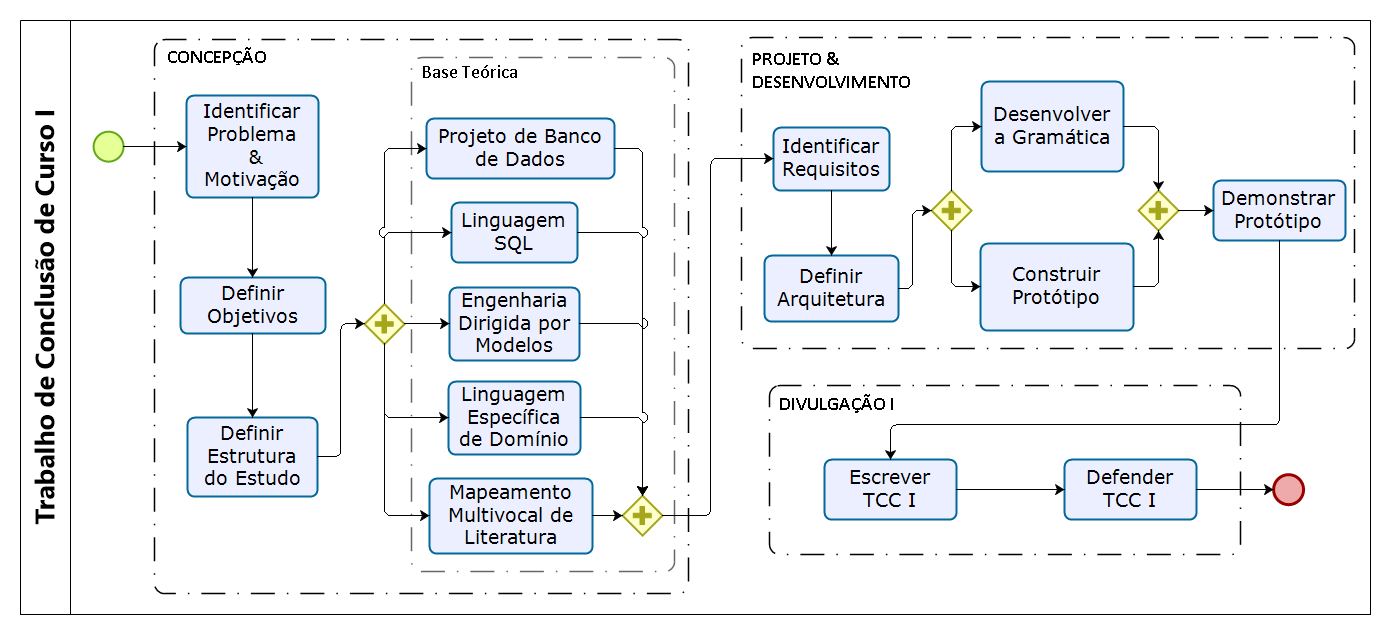
\includegraphics[width=1\textwidth]{img/DesenhoPesquisa1.png}
	\fonte{O autor.}
	\label{fig:ResearchDesign1}
\end{figure}

O projeto foi desenvolvido no \ac{TCC} I, possuindo atividades bem definidas. 
Primeiramente aconteceu o processo de concepção, identificando o problema e a motivação que guiariam todo o estudo. 
Após, foram definidos os objetivos que este trabalho procura atingir. 
Então, houve a elaboração da estrutura geral do estudo em que percebeu-se que era necessário criar uma base teórica bem fundamentada. 
Desta forma, foram caracterizadas as principais áreas que deveriam ser investigadas para o entendimento do domínio do problema. 
Em paralelo, foi realizado um mapeamento multivocal de literatura com o objetivo de encontrar trabalhos similares a esta proposta. 

Com a etapa teórica de concepção realizada, partiu-se então para o projeto inicial da proposta de \ac{DSL}, visando identificar seus requisitos essenciais e sua arquitetura básica. 
Feito isto, deu-se início ao desenvolvimento da descrição de gramática da linguagem e sua implementação de fato. 
Ao fim, um protótipo da ferramenta foi construído. 
A demonstração de uso do protótipo está descrita no Capítulo \autoref{propostaDSL}. 
Como última etapa do \ac{TCC} I, foi realizada a especificação do projeto para a apresentação da proposta.

\begin{figure}[!htb]
	\centering
	\caption{Desenho de pesquisa (continuação).}
		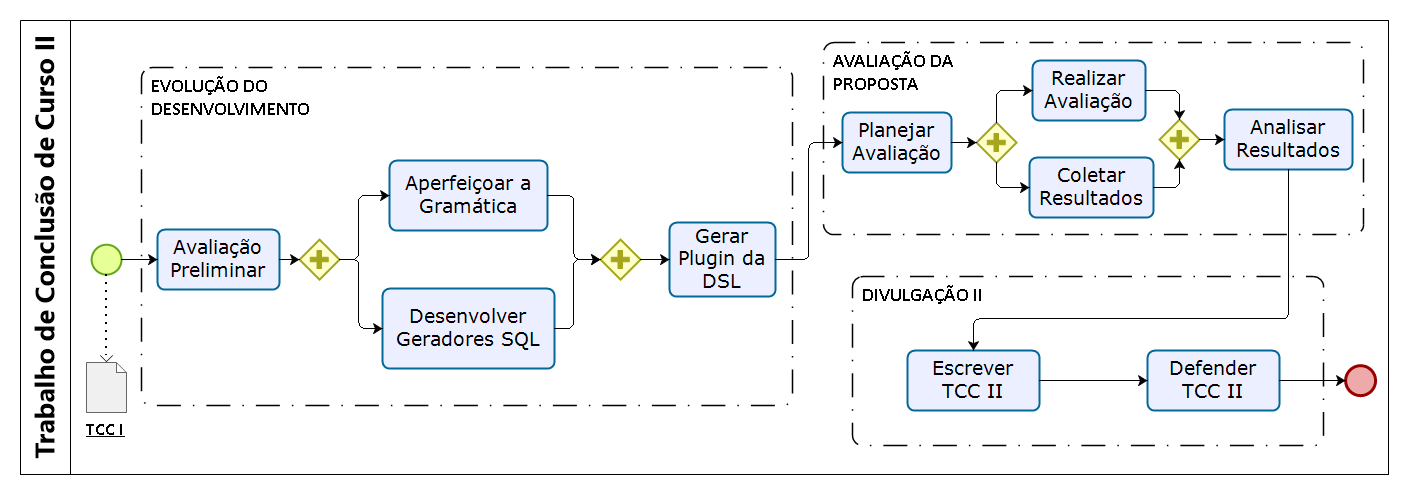
\includegraphics[width=1\textwidth]{img/DesenhoPesquisa2.png}
	\fonte{O autor.}
	\label{fig:ResearchDesign2}
\end{figure}

O \ac{TCC} II tem como entrada os resultados do \ac{TCC} I e inicia-se com uma avaliação preliminar da gramática criada para a \ac{DSL}. 
Após, ocorre a evolução do desenvolvimento, com o aperfeiçoamento da gramática e a construção dos geradores para instruções de Linguagem de Consulta Estruturada, do inglês \ac{SQL}. 
Com essas atividades realizadas, um \textit{plugin} será gerado e incorporado em um \ac{RCP}. 

Com o desenvolvimento finalizado, é desejado que se execute uma avaliação da ferramenta. 
Essa fase vai envolver o planejamento da avaliação para sua realização  e coleta de dados. 
Finalmente, será realizada a análise dos resultados, a escrita do \ac{TCC} II e sua posterior defesa. A \autoref{fig:SinteseTCC} apresenta o resumo geral deste estudo.

% Natureza: 
%     - Pesquisa Aplicada (desenv. procurando gerar uma ferramenta prática para solucionar algo específico)
% Objetivos:
%     - Pesquisa Exploratória (na fase de concepção)
%     - Descritivo (Na fase de avaliação?)
% Procedimentos Técnicos:
%     - Pesquisa Bibliográfica (subfase de base teórica + condução do MSL)
% Abordagem do Problema:
%     - Pesquisa Qualitativa (pela avaliação)

\rowcolors{1}{gray!15}{white}
\begin{table}[!htb]
    \centering
    \caption{Síntese do TCC.}
    \begin{tabular}{m{4.5cm}|m{10cm}}
        \bottomrule
\textbf{Assunto} & Banco de Dados \\
\textbf{Tópico} &  Projeto e Modelagem de Banco de Dados\\
\textbf{Questão de Pesquisa} & Uma \ac{DSL} textual pode auxiliar, em nível conceitual de modelagem, o ensino de projeto e modelagem de banco de dados relacionais? \\
\textbf{Objetivo Principal} & Propor a especificação e realizar a implementação de uma \ac{DSL} para o projeto e modelagem de banco de dados relacionais. \\ 
        \toprule
    \end{tabular}
        \fonte{O autor.}
        \label{fig:SinteseTCC}
\end{table}

%#################################################################
\section{Lições do Capítulo} \label{sec:licMetodo}
%#################################################################


Este capítulo forneceu uma ideia do que é a metodologia de um modo geral e de que forma a pesquisa deste trabalho pode ser classificada. 
Além disso, foi apresentado o desenho estabelecido para a pesquisa, sendo que o que aborda o \ac{TCC} I fornece o entendimento de quais processos foram executados até o momento, e o desenho de \ac{TCC} II aponta o que é  previsto para a sua continuação. 
